\section{Investigation into effect of reliability of stability prediction}
\label{sect:exp_reliability}

\subsection{Introduction} 
As has already been seen in Sect.~\ref{sect:exp_stability}, the choice of length of look-ahead horizon is dependant on the stability of environmental conditions. This experiment is designed to examine what happens if the actual stability is better or worse than that predicted. In such cases the chosen horizon length will be an under-estimate or over-estimate. If $H$ is an under-estimate then we are wasting some of the potential advantage to be had from a long period of stability. If $H$ turns out to be an over-estimate then we might find that the sequence is cut short and we lose some of the groups which had been lined up.

\subsection{Experimental setup}
A simulation was setup using a Phase 2 model containing 500 flexible groups with feasibility windows with lengths from 30 to 120 minutes spread throughout a single night. The model was seeded with 50 groups with scores varying strongly with time over very short (15 minute) feasibility windows. These groups could easily be missed by a despatcher and were intended to boost the performance of look-ahead. A fixed execution timing model was chosen to minimize extraneous random variations.

An environmental model was setup with a 1 hour stability parameter ($\tau_E$). Using a reliability factor $q$ chosen from the range 0.25 to 4.0, the look-ahead horizon was chosen as $H=q\tau_E$ so that $H$ runs from 15 minutes to 4 hours. Where $q<1.0$ this represents an under-estimate while $q>1.0$ represents an over-estimate.  For each $q$ value, 100 simulations were performed with different environmental scenarios generated by the environment model over the selected night and value of $Q_{SU}$ measured. A seperate set of simulations were performed with H set equal to the value of $\tau_E$ and are used as a baseline.

\subsection{Results}
The results of these simulations are plotted in Fig.~\ref{fig:reliable}. The quantity plotted against the y-axis is the ratio $Q_{SU}/Q_0$, with $Q_0$ being the baseline value of $Q_{SU}$ with $H=\tau_E$. The error bars represent variation due to different environmental scenarios on each run. The graphs show a peak value in each case with $q$ around the value of 0.5 to 0.8. Runs with horizon of 0.5 hours show the least variation and no peak. Other horizons show a rapid rise to the peak value then a more gradual fall-off, levelling of to around 0.9 to 0.95 of the baseline value. It is notable that the peak values occur when $q < 1$ which is most likely a feature of the environmental scenario models, the mean and median of the stable period distribution are not equal, with the median being less than $\tau_E$.

\begin{figure}[htp]
\begin{center}
  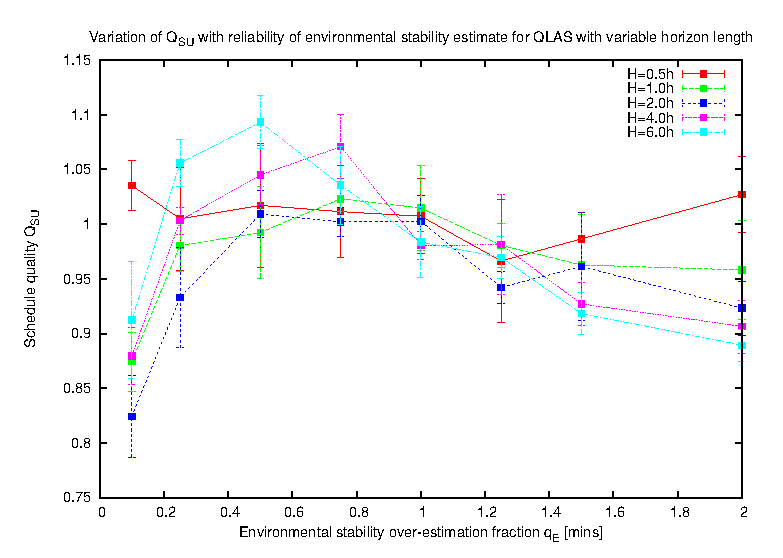
\includegraphics[scale=1.0, angle=0]{figures/horiz_reliability.eps}
  \caption[Variation of qsu with q for different horizon lengths.]
  {Variation of qsu with q for different horizon lengths. For $H=0.5$h there is little effect, whilst longer horizons appear to rise to a peak at $q \sim 0.8$ then a gradual decay, levelling of to around $0.9Q_0$.}
\label{fig:reliable}
\end{center}
\end{figure}
